\documentclass[../Main.tex]{subfiles}
\begin{document}
\chapter{Clean Architecture - A Craftsman's Guide  to Software Structure and Design}

\intro{
    Robert C. Martin
    ISBN-13:	978-0-13-449416-6
    ISBN-10:	0-13-449416-4
}

\section{Comparison}


Requirements:
\begin{itemize}
    \item The most important contents from the book
    \item A personal reflection about the book by the author of the summary
    \item Regular meetings with progress and insights
    \item Atleast 3 meetings
    \item Presentations / slides of the books read by your team. In your final team-meeting, every team
          member must present his/her book using these slides.
    \item Any proof that at least three team-sessions took place, e.g. meeting notes, video recordings, etc.
\end{itemize}

\section{Introduction}

the	rules	of	software	architecture	are
independent	of	every	other	variable.
Wether it is a small or complex system. page 21

Difference between architecture and design -> none at all page 29
The	low-level	details	and	the	high-level
structure	are	all	part	of	the	same	whole.

\defn{Goal}{
    The	goal	of	software	architecture	is	to	minimize	the	human	resources	required	to	build	and
    maintain	the	required	system
}

\begin{figure}[H]
    \centering
    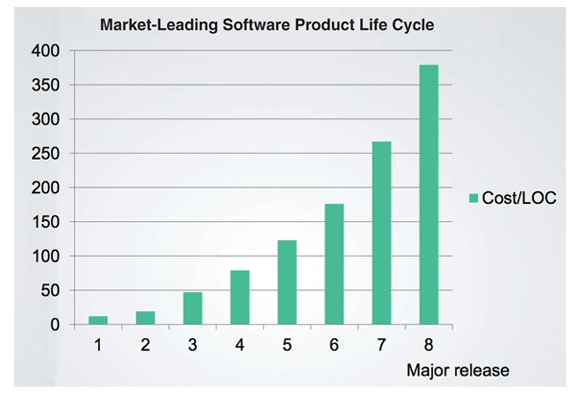
\includegraphics[width=0.75\linewidth]{Images/cpl-over-time.png}
    \caption{Cost per line increases over time due to complexity. More staff is required. This business model in insustainable}
\end{figure}

\begin{itemize}
    \item Take quality seriously. Don't "change later".
\end{itemize}

\section{Values}
%Software provides two values:
%\begin{description}
%    \item[Behavior] How the software meets stakeholder requirements.
%    \item [Structure] how easily the software can be changed.
%\end{description}

Developers ensure both behavior and structure are high.

\begin{description}
    \item[Behavior]
        Developers make machines behave according to requirements.
        Debugging and fixing issues when the behavior deviates.
    \item [Structure]: \begin{description}
              \item [Software] must be "soft" and easy to change.
                    Changes should only depend on scope, not the system's complexity.
                    Over time, changes get harder if the system's architecture isn't flexible.
              \item [Architecture]
                    Needs to be shape-agnostic to allow easy integration of new features.
                    Should not prefer one shape over another, to avoid complex fitting of new features.
          \end{description}
\end{description}

\subsection{Key-Take-Away}
\begin{itemize}
    \item A system with poor architecture can lead to high costs for future changes,
          making it more important for software to be easy to modify than to be initially functional without flexibility.
    \item Focus on both, not just one.
\end{itemize}

\section{Paradigms}

\defn{Structured}{
    Structured	programming	imposes	discipline	on	direct	transfer of	control.
    When dismissing goto statements one could proof programs.
    \begin{itemize}
        \item Proofable Programs is not widely used.
        \item Tests use the "scientific" not the matematical method.
              It proofs something is not wrong, not that something is correct.
        \item Software that is not provable (goto) cannot be deemed correct.
        \item modern	languages	do	not
              typically	support	unrestrained	goto	statements.
        \item functional decomposition
        \item Falsifiable units of programming
    \end{itemize}
    Structured	programming	forces	us	to	recursively	decompose	a	program	into	a	set
    of	small	provable	functions.	We	can	then	use	tests	to	try	to	prove	those	small
    provable	functions	incorrect.	If	such	tests	fail	to	prove	incorrectness,	then	we
    deem	the	functions	to	be	correct	enough	for	our	purposes.

}

\defn{Object Oriented}{
    Object-oriented	programming	imposes	discipline	on	indirect	transfer	of	control.
    \textit{encapsulation,	inheritance,	and	polymorphism}

    OO	is	the	ability,	through	the
    use	of	polymorphism,	to	gain	absolute	control	over	every	source	code
    dependency	in	the	system.	It	allows	the	architect	to	create	a	plugin	architecture,
    in	which	modules	that	contain	high-level	policies	are	independent	of	modules
    that	contain	low-level	details.	The	low-level	details	are	relegated	to	plugin
    modules	that	can	be	deployed	and	developed	independently	from	the	modules
    that	contain	high-level	policies
}

\defn{Functional}{
    Functional	programming	imposes	discipline	upon	assignment.
}

\subsection{Key Take-Away}

\begin{itemize}
    \item Each of the paradigms removes capabilities from the programmer.
    \item Software architects strive to define modules, components, and services that are easily falsifiable (testable).
\end{itemize}

\section{Single Responsibility Principle (SRP)}
S in Solid.
\begin{itemize}
    \item A module should be responsible to	one, and only one, actor.
    \item Misunderstood in the SOLID principle
    \item "module"?	Cohesive set of functions and data structures
\end{itemize}

\begin{figure}[H]
    \centering
    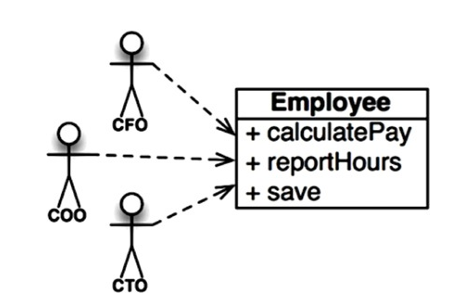
\includegraphics[width=0.75\linewidth]{Images/cleanarch/employee.png}
    \caption{Employee class that has functions for different actors}
\end{figure}

\subsection{Symptoms}
\begin{itemize}
    \item Accidental Duplication
          \begin{itemize}
              \item Accidental change to code which other code within the same module depends on.
          \end{itemize}
    \item Merges
          \begin{itemize}
              \item Actors want to change the same source file
          \end{itemize}
\end{itemize}

\subsection{Solution}
\begin{itemize}
    \item Many different solutions
    \item Seperate data from functions
    \item Put into seperate classes
    \item Use facade
\end{itemize}

\begin{figure}[H]
    \centering
    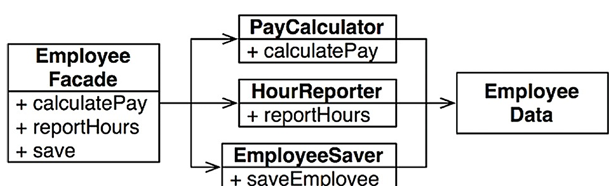
\includegraphics[width=0.75\linewidth]{Images/cleanarch/employeefacade.png}
    \caption{Facade enables easier usage of class. It is responsible for instantiating and delegating.}
\end{figure}

\section{Open-Closed Principle (OCP)}
A software artifact should be open for extension but closed for modification-
\begin{itemize}
    \item Seperate code on how, why and when it changes
    \item Make code hierarchical with the central business logic at the top
    \item If component A should be protected from B, then component B should depend on component A. Use interfaces for this.
\end{itemize}

\begin{figure}[H]
    \centering
    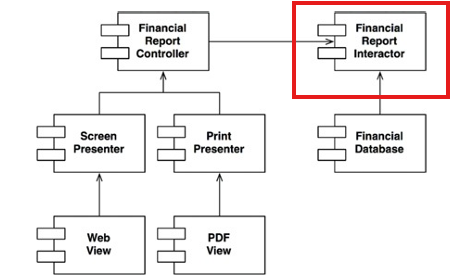
\includegraphics[width=0.75\linewidth]{Images/cleanarch/ocp.png}
    \caption{Abstractions should be structured in a way, so that
        it protects the most important business logic. Here, the lowest
        level is code that interact with the peripherie. It changes the most.}
\end{figure}

\subsection{Playbook}
\begin{itemize}
    \item Partition system into components
    \item \textbf{Arrange components into a dependency hierarchy}
    \item protect higher-level components from changes
\end{itemize}

\section{Liskov Substitution Principle (LSP)}
\begin{figure}[H]
    \centering
    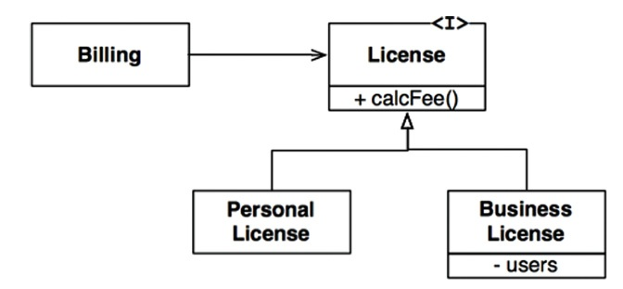
\includegraphics[width=0.75\linewidth]{Images/cleanarch/lsp-example.png}
    \caption{Example of correct subtype. Behaviour of Billing does not depend on the subtype}
\end{figure}
\begin{figure}[H]
    \centering
    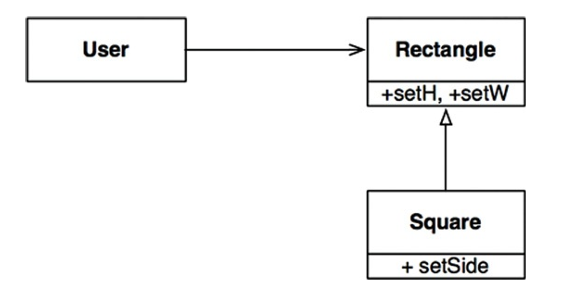
\includegraphics[width=0.75\linewidth]{Images/cleanarch/lsp-wrong-example.png}
    \caption{Example of incorrect usage. The behaviour of the user depends on the types.}
\end{figure}

\subsection{Key Take-Away}
\begin{itemize}
    \item A simple violation of substitutability can cause the architecture to be polluted with extra mechanisms.
\end{itemize}

\section{Interface Segregation Principle (ISP)}
\subsection{Problem}
\begin{figure}[H]
    \centering
    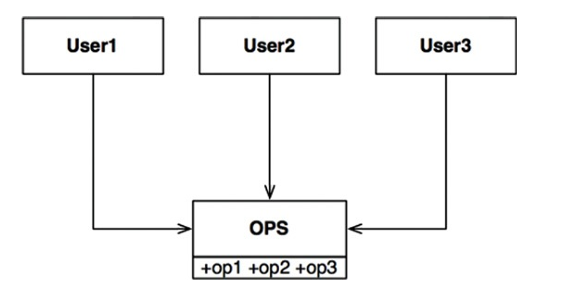
\includegraphics[width=0.75\linewidth]{Images/cleanarch/isp-example-1.png}
    \caption{User1 only uses op1. Since it depends on OPS class it also depends on changes to the op2 and op3 methods}
\end{figure}

\subsection{Solution}
\begin{figure}[H]
    \centering
    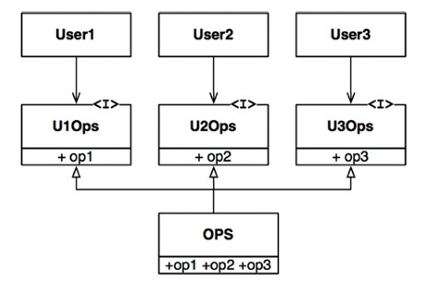
\includegraphics[width=0.75\linewidth]{Images/cleanarch/isp-solution.png}
    \caption{Break behaviour dependencies into multiple interfaces}
\end{figure}

\subsection{Key Take-Away}
\begin{itemize}
    \item Harmful to depend on things you dont need
    \item Do not depend on uneccessary modules
\end{itemize}

\section{Dependency Inversion Principle (DIP)}
Most flexible systems are those in which source code dependencies refer only to abstractions.

We want to avoit depending on volatile concrete elements.
\textbf{We want stable abstractions.}

\begin{itemize}
    \item Don't refer to volatile concrete classes. (Interfaces, Abstract Interfaces)
    \item Don't derive from volatile concrete classes.
    \item Don't override concrete functions.
    \item Never mention the name of anything concrete and volatile.
\end{itemize}

\begin{figure}[H]
    \centering
    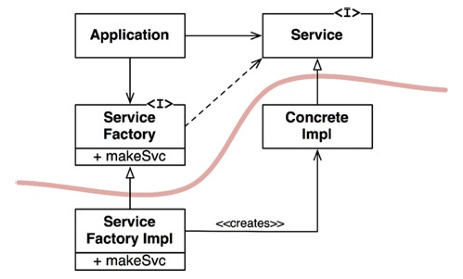
\includegraphics[width=0.75\linewidth]{Images/cleanarch/dip-factory.png}
    \caption{The red line divides the system inabstract and concrete. The flow of control crosses
        the boundary in the opposite direction of the source code dependencies, thats why its called DIP}
\end{figure}

\subsection{Components}

\defn{Components}{
    In this book components refers to:
    \begin{itemize}
        \item Smallest units of deployment
        \item Can be linked together
        \item Can be aggregated into archives
        \item Can be independently deployed as seperate dynamically loaded plugins (e.g DLL)
    \end{itemize}
    We want them to be independently deployable and therefore \textbf{developable}.
}

\section{Component Cohesion}
\begin{figure}[H]
    \centering
    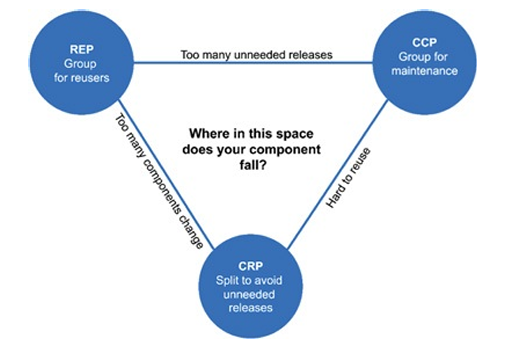
\includegraphics[width=0.75\linewidth]{Images/cleanarch/component-cohesion.png}
\end{figure}

\subsection{Reuse Release Equivalence (REP)}
\begin{itemize}
    \item Classes and modules that are formed into a component must belong to a cohesive group
    \item Overarching theme or purpose
    \item Should be releasable together
          \begin{itemize}
              \item Same Version Number
              \item Release tracking
              \item Release documentation
          \end{itemize}
\end{itemize}

\subsection{Common Closure Principle (CCP)}
\begin{itemize}
    \item Same as SRP but for components
    \item Gather classes that change together
    \item Separate classes to other components if they change for different reasons
\end{itemize}

\subsection{Common Reuse Principle (CRP)}
\begin{itemize}
    \item Dont force users of a component to depend on things they don't need
    \item Classes and modules that tend to be reused together belong in the same component
    \item Classes that are not tightly bound should not be in the same component
\end{itemize}

\section{Component Coupling}
Deal with relationships beteen components.
\subsection{Acyclic Dependencies Principle (ADP)}

\subsubsection{Weekly Build}
Is the practice of isolating devs to work on tasks then integrating at the end of the week.
As the project grows the integration efforts grow.

\subsubsection{Resolution}
\begin{itemize}
    \item Partitioning the development into releasable components.
          Components as units of work can be the responsibility of a single developer or a team.
    \item \textbf{There can be no dependency cycles}
\end{itemize}
\begin{figure}[H]
    \centering
    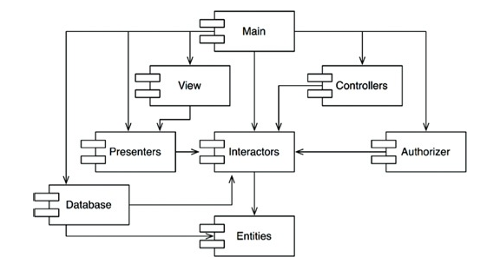
\includegraphics[width=0.75\linewidth]{Images/cleanarch/dependency-cycle.png}
    \caption{Handle dependency acyclic so that changes in components do not affect everything}
\end{figure}

\begin{itemize}
    \item With cycles it is harder to make changes and create unit tests
\end{itemize}

To break the cycle:
\begin{itemize}
    \item Apply Dependency Inversion Principle (DIP)
    \item Create a new component that both components depend on
\end{itemize}

\begin{figure}[H]
    \centering
    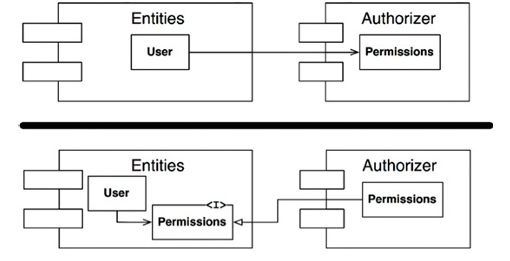
\includegraphics[width=0.75\linewidth]{Images/cleanarch/breaking-the-cycle.png}
\end{figure}

\begin{figure}[H]
    \centering
    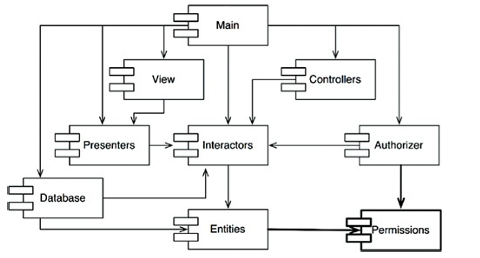
\includegraphics[width=0.75\linewidth]{Images/cleanarch/break-the-cycle-component.png}
\end{figure}

\subsection{Top-Down Design and Component Dependency Graph}
\defn{Component Dependency Graph}{
    Has kittle to do with describing functionality.
    Instead, maps the buildability and maintainability of the application.
    It is not planned at the beginning of the project and evolves.
}

\defn{Stable Dependency Principle}{
    SDP says that the I metric of a component should be larger than the I of the components it depends upon.
}

\subsection{Stability Metrics}
\begin{description}
    \item[Fan In] Incoming dependencies
    \item[Fan Out] Outgoing dependencies
    \item[Instability] \begin{equation}
            I = \frac{\text{Fan-Out}}{\text{Fan-In} + \text{Fan-out}}
        \end{equation}
\end{description}

\subsection{Measuring Abstraction}
\begin{description}
    \item[Nc] Number of classes in component
    \item[Na] Number of abstract classes and interfaces in the component
    \item[A] \begin{equation}
            A = \frac{Na}{Nc}
        \end{equation}
\end{description}

\subsection{Stable Abstraction Principle}
\defn{Stable Abstraction Principle (SAP)}{
    if a component is stable (I=0) it should consist of interfaces and abstract classes,
    so that it can be extendet.
}

\begin{figure}[H]
    \centering
    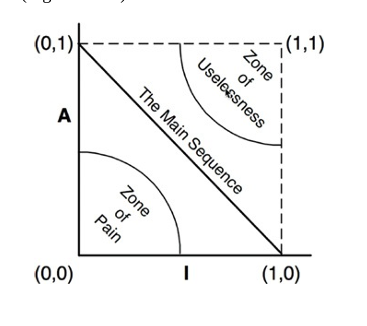
\includegraphics[width=0.75\linewidth]{Images/cleanarch/stable-abstraction-principle.png}
    \caption{
        When plotting A against I we can find zones of exclusion, where components should not be.
        Consider component in the area of (0,0). It is maximaly stable and concrete.
        Such a component is not desirable because it is rigid. The most desirable component sit at the two endpoints of the Main Sequence.
        The Zone near (1,1) is also undesirable berause it is maximally abstract, yet has no dependents thus is useless.
    }
\end{figure}

\subsection{SDP/SAP Important Metric}
D: Distance
\begin{equation}
    D = |A+I-1|
\end{equation}
Ranges from [0,1]. A value of 0 indicates that the component is on the Main Sequence.
A value of 0 indicates the component is far away from the Main Sequence.

\begin{figure}[H]
    \centering
    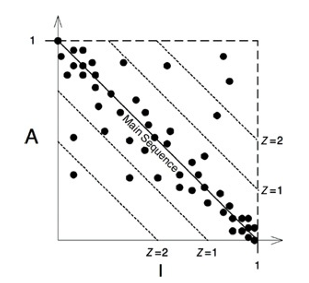
\includegraphics[width=0.75\linewidth]{Images/cleanarch/dependency-scatter.png}
    \caption{
        Dependency Scatter Plot:
        One can create a scatter plot of A and I and compare the different components.
        With this it is shown which components are deviating from the Main Sequence aswell as
        where our median and standard deviation lies.
    }
\end{figure}

\begin{figure}[H]
    \centering
    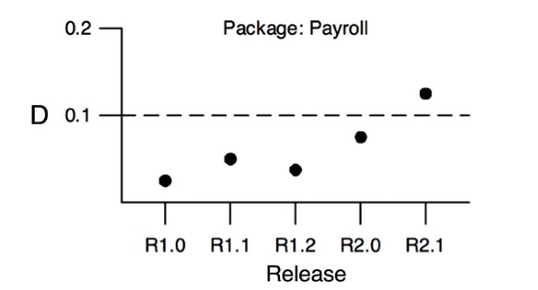
\includegraphics[width=0.75\linewidth]{Images/cleanarch/dependency-evolution.png}
    \caption{
        Dependency Evolution Plot.
        One can also plot the distance metric with a time dimension to see how a component
        deviates from the Main Sequence.
    }
\end{figure}

\section{Architecture}
\defn{Another Definition of Architecture}{
    The primary purpose is to support the life cycle of the system.
    Good architecture makes the system easy to understand, easy to develop, easy to maintain
    and easy to deploy. The ultimate goal is to minimize the lifetime cost of the system and to maximise programmer productivity.
    It must support:
    \begin{itemize}
        \item The use cases and operation
        \item Maintenance
        \item Development
        \item Deployment
    \end{itemize}

    The architecture must not wield much influence over the behavior of the system.
}

\subsection{Drawing Lines}

\begin{figure}[H]
    \centering
    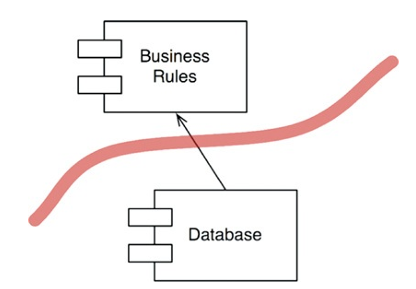
\includegraphics[width=0.75\linewidth]{Images/cleanarch/br-draw-lines.png}
    \caption{
        Draw lines between the business rules and other components.
        Note the direction of the arrow. The Database knows about the br.
        The br do not know about the Database. This implies that the DatabaseInterface live in the br component,
        while the DatabaseAccess classes liuve in the Database component.
        The direction is important. It shows that the Database does not matter to the BusinessRules.
    }
\end{figure}

\begin{figure}[H]
    \centering
    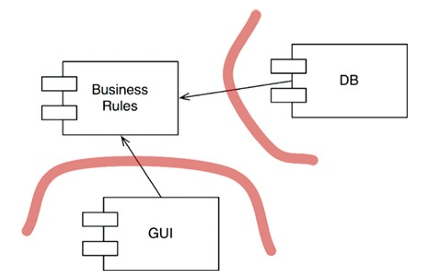
\includegraphics[width=0.75\linewidth]{Images/cleanarch/plugin-br.png}
    \caption{
        It can be desirable to create a architecture where the br does not depend on external components.
        This enables a plugin system.
    }
\end{figure}

\begin{enumerate}
    \item Partition the system into components. Some of those are core business rules, others are plugins that contain necessary functions that are not directly related to the core busines.
    \item Arange the code in those ocmponents such that the arrows between them point in one direction.
\end{enumerate}

\subsection{Policy and Level}

\defn{Level}{
    Defined the distance from the inputs and outputs. The farther a policy is from both, the higher the level.
    We want source code dependencies to be decoupled from data flor and coupled to level.
}

\begin{figure}[H]
    \centering
    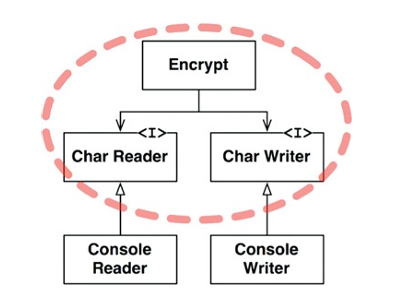
\includegraphics[width=0.75\linewidth]{Images/cleanarch/level.png}
    \caption{
        The component with the highest level should be abstracted from the in and output.
        Note the dashed border. All dependencies crossing that border point inward.
        The lower level components should be plugins.
    }
\end{figure}

\subsection{Business Rules}
\defn{Business Rules}{
    Are rules that make money for the business.
    As critical we define data and rules that would
    exist even when the system was not automated.
}

\defn{Entities}{
    Is an object within our computer system that empodies a small set of critical business rules operating on
    critical business data.
}

\defn{Use Case}{
    Describes an application-specific business rule as opposed to the critical business rules within the entities.
    Use cases contain the rules that specify how and when the critical business rules within the entities are invoked.
    Entities have no knowledgfe of the use cases that control them.
}

\subsection{Screaming Architecture}
Architecture should be "screaming" at first glance what the system is about.
E.g do not conform architecture of a framework like spring.
Frameworks are options to be left open. A good architecture makes it unnecessary to decide on the specific choises early on.
A good architecture makes it easy to change your mind about those decisions. It emphasizes the use cases and decouples them from peripheral concerns.

Example Web Architecture: The choise of web shall not dictate the architecture. It is basicaly and IO device and it should be treated as such,
The system architecture should be as ignorant as possible about how it will be delivered.

\subsection{Clean Architecture}

\begin{figure}[H]
    \centering
    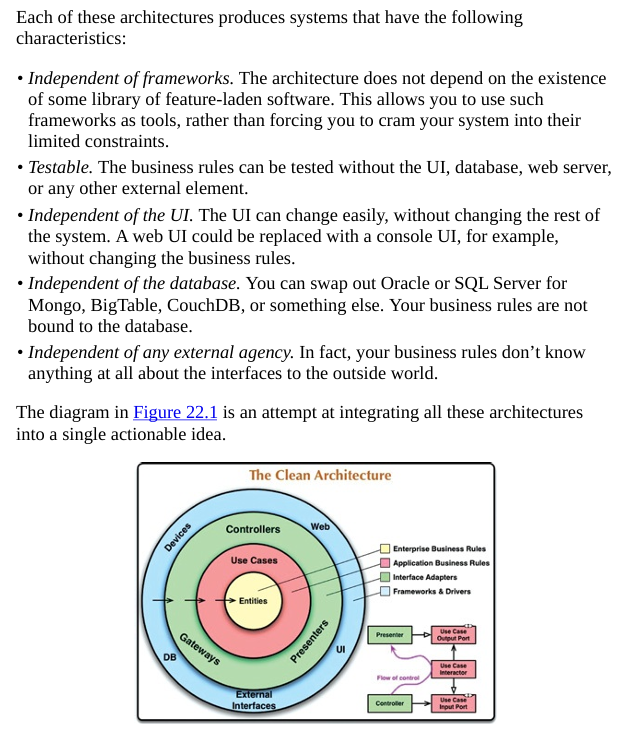
\includegraphics[width=1\linewidth]{Images/cleanarch/clean-architecture.png}
\end{figure}

\subsection{Partial Boundary}
\begin{enumerate}
    \item Implement boundaries as if there were different components. This has high expense but without the burden of versioning.
    \item Use one dimensional boundaries
    \item Facades
\end{enumerate}

\subsection{Main Component}
\begin{itemize}
    \item Only the OS depends on it
    \item Creates all the Factories, Strategies and other global facilities
    \item Hands over control to high-level abstract portions of the system.
    \item Is the dirtiest component
\end{itemize}

\section{Details}
\begin{itemize}
    \item The organizational structure of data, the data model, is architecturally significant
    \item The technologies and systems that move data on and off the devices are not.
    \item The web is a detail.
    \item The GUI is a detail.
    \item Frameworks are details. Solution: Don't marry the framework.
          \begin{itemize}
              \item The frameworks architecture is often not bery clean.
              \item May help you with early features. However, it may outgrow the facilities.
              \item May evolve in a direction that you don't find helpful.
              \item New and better framework may come along.
          \end{itemize}
\end{itemize}

\subsection{Hurdles}
\begin{itemize}
    \item Package By Layer (Horizontal Layering e.g Controller, Service, Data)
          \begin{itemize}
              \item Extremly popular, fast and easy
              \item You may need to modularize down the line
              \item Code structure is not "screaming" and is very similar to others
              \item Most of the time its a relaxed layered architecture. Since there will be
              \item Clear dependencies
              developers that skip dependencies to the next layer. (Controller -> Repo even when planned to use Controller -> Service -> Repo)
          \end{itemize}

    \item Package by Feature (e.g by Feature)
          \begin{itemize}
              \item Typical in DDD. Vertical slicing based on related features, domain concepts or aggregate roots.
              \item Now screams something about the business domain
          \end{itemize}
    \item Ports and Adapters (Onion)
    \begin{itemize}
        \item Business focused
        \item Also screams architecture
        \item Outside components (for infra like UI, DB) depends on the domain not otherway around
    \end{itemize}
    \item Package by Component
    \begin{itemize}
        \item Should mitigate the "big-ball-of-mud" problem. Dependency rules defined by architecture should be checked by the compiler not additional safe keeping.
        \item Hybrid approach
    \end{itemize}
\end{itemize}


\begin{figure}[H]
    \centering
    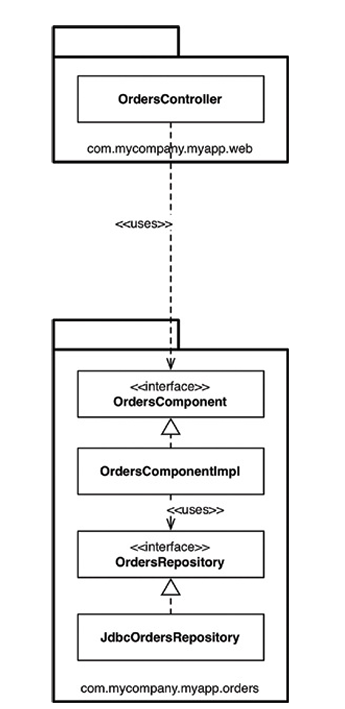
\includegraphics[width=0.5\linewidth]{Images/cleanarch/package-by-components-example.png}
    \caption{An example implementation of "package by components". It uses the definition of components as:
    A grouping of related functionality behind a nice clean interface, which reside inside an execution environment like an application.}
\end{figure}

\newpage

\section{Personal Reflection}

Clean Architecture offers a structured look at how to organize code so it's easier to maintain and adapt over time.
Robert C. Martin lays out familiar ideas, SOLID principles, dependency rules, and component structure in a clear way.
The book is divided into sections that first explain why architecture matters and then show how to apply those principles in a design.
\linebreak
\linebreak
One of the book's strengths is its consistent focus on dependencies.
It repeatedly stresses that if you keep high-level business logic separate from low-level details like frameworks or databases
you reduce the risk of "rippling" changes across the entire codebase.
This advice resonates well: I've seen persons spend a long time untangling intertwined modules, and the book's approach offers some help.
\linebreak
\linebreak
The SOLID principles are presented with simple diagrams and examples.
For someone who has heard these acronyms before, the chapters serve as a useful refresher. If you're newer to these ideas, the book provides a solid introduction without getting too deep into any single topic.
\linebreak
\linebreak
Later chapters introduce component-level principles, how to group classes into cohesive components, avoid cyclic dependencies, and measure stability and abstraction.
These sections feel a bit more theoretical: concepts like "instability" or "main sequence" graphs are interesting but might not be something every team calculates regularly.
Still, the general message is clear, components should change at predictable times, and you want a structure that helps you spot trouble before it grows.
\linebreak
\linebreak
The final parts of the book describe the "Clean Architecture" diagram—layers arranged so that inner circles do not depend on outer circles.
This model echoes ideas found in onion or ports and adapters architectures.
While not every project seems to need such a rigid layering, the diagram serves as a helpful reference when planning a new system or refactoring parts of an existing one.
\linebreak
\linebreak
In practice, following every guideline in the book might feel like overkill for small projects or tight deadlines.
Many teams choose a framework early to get features in front of users quickly, and untangling that decision later can be challenging.
The book acknowledges this risk by advising to "don't marry the framework," but it doesn't go into detail on how to balance that ideal against real-world constraints.
That said, even if you can't apply every idea, the book's vocabulary and emphasis on clear boundaries give you points to discuss when reviewing code or planning a sprint.
\linebreak
\linebreak
Overall, Clean Architecture strikes a balance between high-level theory and practical advice.
It doesn't promise magic fixes, but it does offer a mindset, think ahead about how code will grow, and avoid letting details like a particular web framework dictate your core logic.

\end{document}